% Compile: tectonic slides/submission.tex --outdir output/final
\documentclass[aspectratio=169,11pt]{beamer}
\usepackage{fontspec,amsmath,amssymb,booktabs,tikz,listings,etoolbox,graphicx}
\IfFontExistsTF{Arial}{\setsansfont{Arial}}{\setsansfont{lmsans10-regular.otf}[BoldFont=lmsans10-bold.otf,ItalicFont=lmsans10-oblique.otf]}
\setmonofont{lmmono10-regular.otf}[Scale=.9]
\usetikzlibrary{arrows.meta,positioning,calc}
% Fill in current team details before submission. Do not reuse the sample's authors.
\newcommand{\CourseName}{INTRODUCTION TO ARTIFICIAL INTELLIGENCE}
\newcommand{\CourseCode}{CO3061}
\newcommand{\Semester}{261}
\newcommand{\ReportMonth}{Tháng 10 năm 2026}
\newcommand{\InstructorName}{Ths. Vương Bá Thịnh}
% Example: Họ tên thứ nhất & MSSV thứ nhất & Lớp thứ nhất \\ Họ tên thứ hai & MSSV thứ hai & Lớp thứ hai
\newcommand{\StudentRows}{Hà Bảo Nhi & 2312496 & (L01) \\ Lê Chí Đại & 2310621 & (L01) \\ Đào Quang Dương & 2310579 & (L01) \\ Lương Minh Thuận & 2313348 & (L02) \\ Nguyễn Quốc Huy & 2311209 & (L02)}

\usetheme{HCMUT}
\definecolor{ink}{HTML}{25282D}
\definecolor{water}{HTML}{258BD2}
\definecolor{muted}{HTML}{637284}
\lstset{basicstyle=\ttfamily\footnotesize,columns=fullflexible,keepspaces=true,
showstringspaces=false,breaklines=true,keywordstyle=\color{HCMUTblue},
morekeywords={if,for,while,return,in,or},aboveskip=3pt,belowskip=3pt}
\newcommand{\slidenote}[1]{\par\vspace{2mm}{\scriptsize\color{muted}#1\par}}
\newcommand{\tile}[4]{\begin{scope}[shift={(#1,#2)}]
\draw[black!20](-.5,-.5)rectangle(.5,.5);
\foreach \bit/\dx/\dy in {1/0/.5,2/.5/0,4/0/-.5,8/-.5/0}{
\pgfmathtruncatemacro{\hasport}{mod(floor(#3/\bit),2)}
\ifnum\hasport=1\draw[#4,line width=3.6pt,line cap=round](0,0)--(\dx,\dy);\fi}
\end{scope}}
\newcommand{\board}[2]{\foreach \mask[count=\idx from 0] in {#1}{
\pgfmathtruncatemacro{\col}{mod(\idx,4)}\pgfmathtruncatemacro{\row}{-floor(\idx/4)}
\tile{\col}{\row}{\mask}{#2}}\fill[white](2,-2)circle(.16);\fill[HCMUTblue](2,-2)circle(.11);}
\hypersetup{pdftitle={BTL1: Pipes va Light Up},pdfsubject={Tim kiem - CO3061}}
\begin{document}

\begin{frame}[plain]
\begin{columns}[c,onlytextwidth]
\column{.18\textwidth}\centering
\includegraphics[height=18mm]{../report/assets/hcmut-logo.png}
\column{.79\textwidth}\small\color{HCMUTblue}
ĐẠI HỌC QUỐC GIA THÀNH PHỐ HỒ CHÍ MINH\par
TRƯỜNG ĐẠI HỌC BÁCH KHOA\par
KHOA KHOA HỌC VÀ KỸ THUẬT MÁY TÍNH
\end{columns}
\vspace{5mm}{\color{HCMUTblue}\hrule}\vspace{5mm}
{\Large\bfseries BÀI TẬP LỚN 1: TÌM KIẾM\par}
\vspace{3mm}{\LARGE\bfseries Pipes và Light Up\par}
\vspace{3mm}Nhập môn Trí tuệ nhân tạo (\CourseCode)\par
{\small Học kỳ 1, năm học 2026--2027\par}
\vspace{3mm}
\ifdefempty{\InstructorName}{}{\small Giảng viên: \InstructorName\par}
\ifdefempty{\ClassName}{}{\small Lớp: \ClassName\par}
\ifdefempty{\StudentRows}{}{\small\begin{tabular}{@{}ll@{}}\StudentRows\end{tabular}}
\end{frame}

\begin{frame}{Nội dung}
\begin{columns}[T,onlytextwidth]
\column{.49\textwidth}\tableofcontents[sections={1}]
\column{.49\textwidth}\tableofcontents[sections={2}]
\end{columns}
\vspace{3mm}\small Mỗi game: một giải thuật mù, một giải thuật heuristic, demo từng bước và bảng đo thời gian/bộ nhớ.
\end{frame}

\section{Pipes}
\subsection{Giới thiệu}
\begin{frame}{Giới thiệu}
\begin{columns}[c,onlytextwidth]
\column{.39\textwidth}\centering
\begin{tikzpicture}[scale=.85]
\board{2,12,2,12,4,5,4,5,7,11,15,13,3,8,1,1}{water}
\end{tikzpicture}
\slidenote{Một nghiệm của pipes-4x4-261.}
\column{.57\textwidth}
\begin{itemize}
\item Xoay từng ống; hình dạng ống giữ nguyên.
\item Các cổng phải khớp nhau, không mở ra ngoài biên.
\item Mọi ô nối thành một mạng, không có chu trình.
\end{itemize}
\vspace{3mm}\textbf{Hai giải thuật:} DFS và Greedy Best-First.
\end{columns}
\end{frame}

\subsection{Phát biểu bài toán tìm kiếm}
\begin{frame}{Phát biểu bài toán tìm kiếm}
\small\begin{tabular}{@{}p{.22\textwidth}p{.73\textwidth}@{}}\toprule
Thành phần & Biểu diễn\\\midrule
Trạng thái & $s=(a_0,\ldots,a_{k-1})$: hướng đã gán cho $k$ ô đầu\\
Ban đầu & $()$, chưa gán hướng cho ô nào\\
Hành động & Gán một hướng cho ô $k$, theo thứ tự hàng--cột\\
Đích & Gán đủ $n=m^2$ ô và mạng thỏa luật\\
Không gian & $\prod_i |R_i|\leq4^n$ cấu hình trước kiểm tra ràng buộc\\\bottomrule
\end{tabular}
\vspace{3mm}\par
Ống thẳng có 2 hướng; chữ thập có 1; các hình còn lại có 4.\par
Giải thuật gán thẳng hướng cuối cho một ô (bằng 0--3 lần nhấp xoay).
\end{frame}

\subsection{Tạo dữ liệu đầu vào}
\begin{frame}{Tạo dữ liệu đầu vào}
\begin{center}\begin{tikzpicture}[node distance=5mm,
box/.style={draw=HCMUTblue,align=center,font=\small,minimum height=9mm}]
\node[box,text width=38mm](a){Sinh mạng cây trên lưới};
\node[box,text width=35mm,right=of a](b){Xoay ngẫu nhiên từng ống};
\node[box,text width=33mm,right=of b](c){Lưu bản đồ JSON};
\draw[-{Stealth}](a)--(b);\draw[-{Stealth}](b)--(c);
\end{tikzpicture}\end{center}
\begin{itemize}
\item 9 bản: $4\times4$, $5\times5$, $7\times7$; mỗi cỡ 3 seed.
\item JSON lưu kích thước, nguồn và ma trận cổng N/E/S/W.
\item Mạng cây bảo đảm có nghiệm; solver không đọc đáp án lúc sinh.
\end{itemize}
\slidenote{Luật và dạng ống lấy theo puzzle-pipes.com; bàn do chương trình tự sinh.}
\end{frame}

\subsection{Giải thuật tìm kiếm mù}
\begin{frame}[fragile]{Giải thuật tìm kiếm mù: DFS}
\begin{columns}[T,onlytextwidth]
\column{.57\textwidth}
\begin{lstlisting}
DFS(s):
  if limit reached: return LIMIT
  if GOAL(s): return SOLVED(s)
  for a in rotations of tile |s|:
    child = s + (a)
    if FEASIBLE(child):
      result = DFS(child)
      if solved or limited:
        return result
  return UNSOLVABLE
\end{lstlisting}
\column{.39\textwidth}\small
Đi sâu theo thứ tự cố định; bế tắc thì quay lui.\par\vspace{2mm}
\textbf{Cắt tỉa dùng chung:}
\begin{itemize}
\item Cổng vượt biên.
\item Không khớp ô đã gán.
\item Đã tạo chu trình.
\item Không thể nối hết ô.
\end{itemize}
\end{columns}
\slidenote{Kiểm tra ở gốc: tổng số cổng phải bằng $2(n-1)$ vì mạng là một cây.}
\end{frame}

\subsection{Giải thuật tìm kiếm heuristic}
\begin{frame}[fragile]{Giải thuật tìm kiếm heuristic: Greedy Best-First}
\[h(s)=\sum_{i\text{ chưa gán}}\log_2|D_i(s)|\]
\small $D_i(s)$ là miền hướng còn lại của ô $i$. Ưu tiên $h$ nhỏ hơn.\par
Ví dụ: miền $(1,2,4)$ cho $h=3$; miền $(1,1,2)$ cho $h=1$.
\begin{lstlisting}
push root into min-heap
while heap not empty:
  s = pop state with lowest priority
  if GOAL(s): return SOLVED(s)
  for child in feasible successors(s):
    push (h(child), -depth(child), serial, child)
return UNSOLVABLE
\end{lstlisting}
\slidenote{Cùng thứ tự ô và cắt tỉa với DFS; chỉ khác thứ tự lấy trạng thái ra. Hòa $h$ thì chọn trạng thái sâu hơn.}
\end{frame}

\subsection{Hiện thực và minh họa từng bước}
\begin{frame}{Hiện thực và minh họa từng bước}
\begin{columns}[c,onlytextwidth]
\column{.37\textwidth}\centering
\begin{tikzpicture}[scale=.77]
\board{2,9,1,6,4,5,1,10,14,13,15,7,6,4,2,4}{muted}
\draw[HCMUTblue,line width=1.3pt](.5,.5)rectangle(1.5,-.5);
\end{tikzpicture}
\column{.59\textwidth}\small
Ví dụ bước gán ô thứ hai:
\begin{enumerate}
\item Ô đầu có cổng Đông.
\item Thử ES ở ô kế: thiếu cổng Tây $\Rightarrow$ loại.
\item Thử SW: khớp ô đầu $\Rightarrow$ đi tiếp.
\end{enumerate}
\vspace{2mm}Trên game: chọn DFS/Greedy, dùng Run, Pause, Next; xem lý do loại nhánh và Show solution.
\end{columns}
\slidenote{Python 3, pygame-ce. Luật ở model.py; giải thuật ở search.py; giao diện ở app.py.}
\end{frame}

\subsection{Kết quả thực nghiệm}
\begin{frame}{Kết quả thực nghiệm}
% Source: docs/benchmarks/2026-10-25-pipes.csv, successful-run group medians (Linux, 25 Oct 2026).
\begin{center}
\small
\begin{tabular}{@{}llrrr@{}}
\toprule
Size & Algorithm & Solved/runs & Time (ms) & Peak (KiB)\\
\midrule
$4\times4$ & DFS    & 15/15 & 3.149  & 26.984\\
           & Greedy & 15/15 & 3.097  & 12.359\\
$5\times5$ & DFS    & 15/15 & 5.261  & 53.297\\
           & Greedy & 15/15 & 6.157  & 19.219\\
$7\times7$ & DFS    & 15/15 & 24.469 & 145.852\\
           & Greedy & 15/15 & 31.695 & 27.594\\
\bottomrule
\end{tabular}
\end{center}

\small 9 bản $\times$ 2 giải thuật $\times$ 5 lần lặp = 90 lượt, đều giải được.\par
Giới hạn mỗi lượt: 30 giây và 200.000 lần mở rộng.
\slidenote{Trung vị theo cỡ bàn. Thời gian đo không vẽ giao diện; bộ nhớ là đỉnh cấp phát Python (tracemalloc). Bảng từng bàn trong báo cáo.}
\end{frame}

\subsection{Nhận xét}
\begin{frame}{Nhận xét}
\begin{itemize}
\item Hai giải thuật nhanh gần bằng nhau; DFS nhỉnh hơn ở $5\times5$ và $7\times7$.
\item Lý do: cắt tỉa đã loại gần hết hướng sai, DFS gần như đi thẳng tới nghiệm. Greedy còn tốn thời gian tính $h$ và thao tác heap.
\item Greedy dùng ít bộ nhớ hơn 2--5 lần: heap rất nhỏ, còn DFS giữ bản sao trạng thái ở mỗi mức.
\end{itemize}
\vspace{3mm}\textbf{Hạn chế:} mới có 9 bàn khá dễ, chưa có bàn vô nghiệm trong bảng đo.
\end{frame}

\section{Light Up (Akari)}
\subsection{Giới thiệu}
\begin{frame}{Giới thiệu}
\begin{columns}[c,onlytextwidth]
\column{.36\textwidth}\centering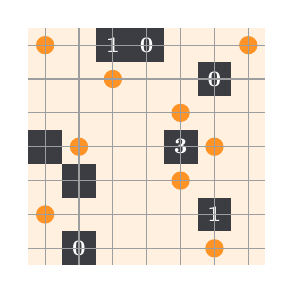
\begin{tikzpicture}[scale=.43]
\fill[orange!12] (-.5,.5) rectangle (6.5,-6.5);
\fill[ink!90] (2-.5,-0-.5) rectangle (2+.5,-0+.5);
\node[white,font=\footnotesize\bfseries] at (2,-0) {1};
\fill[ink!90] (3-.5,-0-.5) rectangle (3+.5,-0+.5);
\node[white,font=\footnotesize\bfseries] at (3,-0) {0};
\fill[ink!90] (5-.5,-1-.5) rectangle (5+.5,-1+.5);
\node[white,font=\footnotesize\bfseries] at (5,-1) {0};
\fill[ink!90] (0-.5,-3-.5) rectangle (0+.5,-3+.5);
\fill[ink!90] (4-.5,-3-.5) rectangle (4+.5,-3+.5);
\node[white,font=\footnotesize\bfseries] at (4,-3) {3};
\fill[ink!90] (1-.5,-4-.5) rectangle (1+.5,-4+.5);
\fill[ink!90] (5-.5,-5-.5) rectangle (5+.5,-5+.5);
\node[white,font=\footnotesize\bfseries] at (5,-5) {1};
\fill[ink!90] (1-.5,-6-.5) rectangle (1+.5,-6+.5);
\node[white,font=\footnotesize\bfseries] at (1,-6) {0};
\fill[orange!85] (0,-0) circle (.27);
\fill[orange!85] (6,-0) circle (.27);
\fill[orange!85] (2,-1) circle (.27);
\fill[orange!85] (4,-2) circle (.27);
\fill[orange!85] (1,-3) circle (.27);
\fill[orange!85] (5,-3) circle (.27);
\fill[orange!85] (4,-4) circle (.27);
\fill[orange!85] (0,-5) circle (.27);
\fill[orange!85] (5,-6) circle (.27);
\draw[ink!45] (-.5,.5) grid (6.5,-6.5);
\end{tikzpicture}

\column{.60\textwidth}\begin{itemize}
\item Đặt bóng trên ô trắng, chiếu theo hàng/cột đến tường.
\item Mọi ô trắng phải sáng.
\item Hai bóng không nhìn thấy nhau.
\item Tường số có đúng số bóng kề trực tiếp.
\end{itemize}\vspace{3mm}
\textbf{Hai giải thuật:} DFS và CSP (backtracking + MRV + CP).
\end{columns}
\slidenote{Luật theo Nikoli. Hình: bàn $7\times7$ seed 70097 và lời giải CSP tìm được.}
\end{frame}

\subsection{Phát biểu bài toán tìm kiếm}
\begin{frame}{Phát biểu bài toán tìm kiếm}
\small\begin{tabular}{@{}p{.22\textwidth}p{.73\textwidth}@{}}\toprule
Thành phần & Biểu diễn\\\midrule
Trạng thái & Tập bóng, ô sáng và vị trí còn hợp lệ (bitmask)\\
Ban đầu & Chưa có bóng; CSP có thể suy ra bóng ngay tại gốc\\
Hành động & Đặt bóng; CSP có thể chọn một tổ hợp quanh tường\\
Đích & Sáng hết ô trắng, không xung đột, mọi số trên tường đúng\\
Không gian & $2^W$ tập bóng trước ràng buộc, với $W$ ô trắng\\\bottomrule
\end{tabular}
\vspace{3mm}\par
Một nút CSP có thể đặt nhiều bóng cùng lúc nhờ suy luận.\par
Cả hai tìm lời giải đầu tiên, không tối ưu số bóng.
\end{frame}

\subsection{Tạo dữ liệu đầu vào}
\begin{frame}{Tạo dữ liệu đầu vào}
\begin{enumerate}
\item Dùng seed chọn vị trí tường.
\item Đặt bóng làm chứng đến khi mọi ô trắng sáng.
\item Suy ra số trên tường; giữ một phần tường không số.
\item Kiểm chứng lời giải làm chứng trước khi trả bàn.
\end{enumerate}
\vspace{3mm}\small
4 cỡ: $7,10,14,25$; 3 nhãn; 5 seed khác nhau mỗi cấu hình.\par
Tổng cộng \textbf{60 bản}, mỗi bản dùng chung cho hai giải thuật.
\slidenote{easy/normal/hard khác nhau ở tỉ lệ tường: 16\%, 10.5\%, 5.5\%. Solver không biết lời giải mẫu.}
\end{frame}

\subsection{Giải thuật tìm kiếm mù}
\begin{frame}[fragile]{Giải thuật tìm kiếm mù: DFS}
\begin{lstlisting}
DFS(state):
  if limit reached: return LIMIT
  if GOAL(state): return SOLVED
  target = first dark cell in row-major order
  for bulb in legal illuminators(target):
    child = place(bulb)
    if FEASIBLE(child):
      result = DFS(child)
      if solved or limited: return result
    exclude bulb from later sibling choices
  return UNSOLVABLE
\end{lstlisting}
\small Đi sâu theo thứ tự cố định. Loại nhánh nếu tường không đủ chỗ hoặc ô tối không còn nguồn chiếu.
\slidenote{Trong code, đệ quy được thay bằng stack tường minh.}
\end{frame}

\subsection{Giải thuật tìm kiếm heuristic}
\begin{frame}{CP: suy luận trước khi chọn nhánh}
\begin{columns}[c,onlytextwidth]
\column{.34\textwidth}\centering
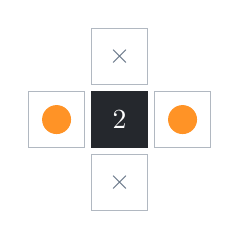
\begin{tikzpicture}[scale=.8]
\foreach \x/\y in {-1/0,1/0,0/1,0/-1}{\draw[muted!50](\x-.45,\y-.45)rectangle(\x+.45,\y+.45);}
\fill[ink](-.45,-.45)rectangle(.45,.45);\node[white]at(0,0){2};
\fill[orange!85](-1,0)circle(.23);\fill[orange!85](1,0)circle(.23);
\node[muted]at(0,1){$\times$};\node[muted]at(0,-1){$\times$};
\end{tikzpicture}\slidenote{Tường đủ 2 bóng: cấm hai ô kề còn lại.}
\column{.62\textwidth}\small
\textbf{\texttt{PROPAGATE}: lặp đến khi không đổi}
\begin{itemize}
\item Tường đủ bóng: cấm các ô kề còn lại.
\item Tường thiếu $r$ bóng, còn đúng $r$ ô: đặt tất cả.
\item Ô tối còn một nguồn chiếu: đặt bóng tại đó.
\item Bóng mới cấm các vị trí nhìn thấy nó; loại ô gây thiếu chỗ quanh tường.
\end{itemize}
\vspace{2mm}Mâu thuẫn $\Rightarrow$ quay lui. Chưa xong $\Rightarrow$ MRV.
\end{columns}
\slidenote{Trạng thái dùng chung: \texttt{(bulbs, lit, legal)} = tập bóng, ô sáng, vị trí còn được phép đặt.}
\end{frame}

\begin{frame}{MRV: chọn ràng buộc có điểm nhỏ nhất}
\begin{columns}[T,onlytextwidth]
\column{.48\textwidth}
\begin{block}{Tường số $w$}
\small $r=k_w-|N(w)\cap bulbs|$: bóng còn thiếu.\par
$u=|N(w)\cap legal|$: ô kề còn được đặt.
\[
 m_{\mathrm{wall}}(w)=\binom{u}{r},\quad r>0
\]
\centering $u=3,\ r=2\ \Rightarrow\ \boxed{m=3}$
\end{block}
\column{.48\textwidth}
\begin{block}{Ô tối $i$}
\small $C(i)=V(i)\cap legal$: các nguồn chiếu.\par
$V(i)$ gồm cả ô $i$.
\[
 m_{\mathrm{dark}}(i)=|C(i)|
\]
\centering Hai nguồn chiếu $\Rightarrow\ \boxed{m=2}$
\end{block}
\end{columns}
\vspace{2mm}\centering
\textbf{Chọn ô tối: $2<3$. Bằng điểm thì ưu tiên tường.}
\slidenote{$N(w)$: ô trắng kề tường; $k_w$: số trên tường. Điểm tường tính trước khi loại tổ hợp bóng chiếu nhau; có thể khác số nhánh thực tế.}
\end{frame}

\begin{frame}{Gain: thử nhánh chiếu sáng thêm nhiều ô trước}
\small Sau khi chọn ràng buộc bằng MRV, xếp nhánh theo
$gain(A)=|(\bigcup_{b\in A}V(b))\cap dark|$ giảm dần.
\begin{columns}[T,onlytextwidth]
\column{.48\textwidth}\centering
\textbf{Nhánh 1: đặt $(7,7)$, gain = 7}\par\vspace{1mm}
\begin{tikzpicture}[x=.35cm,y=-.35cm,font=\tiny]
% Snapshot after root CP: 7x7 easy, seed 70098; coordinates below are zero-based.
\foreach \c/\r in {0/0,2/0,3/0,4/0,5/0,6/0,2/1,3/1,4/1,6/1,0/2,1/2,3/2,4/2,5/2,0/3,1/3,2/3,3/3,4/3,5/3,6/3,0/4,2/4,5/4,0/5,2/5,0/6,2/6}{\fill[orange!12] (\c,\r) rectangle ++(1,1);}
\foreach \c/\r in {6/4,6/5,1/6,3/6,4/6,5/6,6/6}{\fill[HCMUTblue!30] (\c,\r) rectangle ++(1,1);}
\foreach \c/\r/\n in {1/0/-1,0/1/2,1/1/1,5/1/3,2/2/2,6/2/-1,1/5/0,5/5/0}{
  \fill[ink] (\c,\r) rectangle ++(1,1);
  \ifnum\n>-1\node[white] at (\c+.5,\r+.5) {\n};\fi}
\foreach \i in {0,...,7}{
  \draw[muted!40,thin] (\i,0)--(\i,7);
  \draw[muted!40,thin] (0,\i)--(7,\i);}
\foreach \c/\r in {0/0,5/0,2/1,6/1,0/2,5/2,2/3}{\fill[orange!85!black] (\c+.5,\r+.5) circle (.16);}
\fill[HCMUTblue] (6.5,6.5) circle (.22);
\draw[red!80!black,very thick] (6.08,5.08) rectangle (6.92,5.92);
\foreach \i in {0,...,6}{
  \pgfmathtruncatemacro{\labelnum}{\i+1}
  \node[muted] at (\i+.5,-.35) {\labelnum};
  \node[muted] at (-.35,\i+.5) {\labelnum};}
\end{tikzpicture}
\column{.48\textwidth}\centering
\textbf{Nhánh 2: đặt $(5,7)$, gain = 6}\par\vspace{1mm}
\begin{tikzpicture}[x=.35cm,y=-.35cm,font=\tiny]
% Snapshot after root CP: 7x7 easy, seed 70098; coordinates below are zero-based.
\foreach \c/\r in {0/0,2/0,3/0,4/0,5/0,6/0,2/1,3/1,4/1,6/1,0/2,1/2,3/2,4/2,5/2,0/3,1/3,2/3,3/3,4/3,5/3,6/3,0/4,2/4,5/4,0/5,2/5,0/6,2/6}{\fill[orange!12] (\c,\r) rectangle ++(1,1);}
\foreach \c/\r in {1/4,3/4,4/4,6/4,6/5,6/6}{\fill[HCMUTblue!30] (\c,\r) rectangle ++(1,1);}
\foreach \c/\r/\n in {1/0/-1,0/1/2,1/1/1,5/1/3,2/2/2,6/2/-1,1/5/0,5/5/0}{
  \fill[ink] (\c,\r) rectangle ++(1,1);
  \ifnum\n>-1\node[white] at (\c+.5,\r+.5) {\n};\fi}
\foreach \i in {0,...,7}{
  \draw[muted!40,thin] (\i,0)--(\i,7);
  \draw[muted!40,thin] (0,\i)--(7,\i);}
\foreach \c/\r in {0/0,5/0,2/1,6/1,0/2,5/2,2/3}{\fill[orange!85!black] (\c+.5,\r+.5) circle (.16);}
\fill[HCMUTblue] (6.5,4.5) circle (.22);
\draw[red!80!black,very thick] (6.08,5.08) rectangle (6.92,5.92);
\foreach \i in {0,...,6}{
  \pgfmathtruncatemacro{\labelnum}{\i+1}
  \node[muted] at (\i+.5,-.35) {\labelnum};
  \node[muted] at (-.35,\i+.5) {\labelnum};}
\end{tikzpicture}
\end{columns}
\slidenote{Seed 70098, sau CP ở gốc. Viền đỏ: ô tối $(6,7)$ có hai nguồn chiếu. Chấm cam: bóng đã đặt; chấm xanh: bóng thử; nền xanh: ô mới sáng.}
\small\textbf{Thử $(7,7)$ trước $(5,7)$.} Đếm mỗi ô một lần, trước CP của con.
\slidenote{Gain không cộng vào điểm MRV. Nhánh 2 cấm nguồn $(7,7)$ đã thử ở nhánh 1.}
\end{frame}

\begin{frame}[fragile]{Backtracking: CP $\rightarrow$ MRV/gain $\rightarrow$ thử nhánh}
\begin{lstlisting}[basicstyle=\ttfamily\scriptsize]
BACKTRACK_MRV_CP(state):
  if budget exhausted: return LIMIT
  state, ok = PROPAGATE(state)
  if not ok: return UNSOLVABLE
  if GOAL(state): return SOLVED(state)
  checkpoint = state
  choices = SELECT_MRV_CHOICES(checkpoint)
  for child in choices:  # descending gain, before child CP
    result = BACKTRACK_MRV_CP(child)
    if result is SOLVED or LIMIT: return result
    state = checkpoint
  return UNSOLVABLE
\end{lstlisting}
\slidenote{\texttt{SELECT\_MRV\_CHOICES}: chọn ràng buộc, sinh nhánh và xếp gain. Checkpoint giữ đủ \texttt{(bulbs, lit, legal)} sau CP của cha. Code dùng stack thay đệ quy.}
\end{frame}

\subsection{Hiện thực và minh họa từng bước}
\begin{frame}{Hiện thực và minh họa từng bước}
\begin{enumerate}
\item Chọn DFS hoặc CSP, bấm Start Search.
\item Pause và hai mũi tên để đi tới/lui từng bước.
\item CSP hiện thêm bóng suy ra, ô bị cấm $\times$ và lúc quay lui.
\item Compare DFS and CSP: chạy cả hai trên bàn đang mở.
\end{enumerate}
\vspace{3mm}\small
Solver chạy trong worker riêng; giao diện nhận từng sự kiện để vẽ.
\slidenote{Python 3, pygame-ce. Luật ở core/, giải thuật ở algorithms/search.py, giao diện ở ui/app.py.}
\end{frame}

\subsection{Kết quả thực nghiệm}
\begin{frame}{Kết quả thực nghiệm: số bản giải được}
\centering\small\begin{tabular}{@{}lrrrr@{}}\toprule
 & \multicolumn{2}{c}{DFS} & \multicolumn{2}{c}{CSP}\\
Cỡ & Giải được & TIMEOUT & Giải được & TIMEOUT\\\midrule
$7\times7$ & 15/15 & 0 & 15/15 & 0\\
$10\times10$ & 15/15 & 0 & 15/15 & 0\\
$14\times14$ & 15/15 & 0 & 15/15 & 0\\
$25\times25$ & 7/15 & 8 & 15/15 & 0\\\midrule
Tổng & 52/60 & 8 & 60/60 & 0\\\bottomrule
\end{tabular}\par\vspace{3mm}
\raggedright 60 bản $\times$ 2 giải thuật = 120 lượt. Mỗi bản đo một lần mỗi giải thuật.\par
Giới hạn: 30 giây, 500.000 node, 512 MiB ước lượng.
\slidenote{Mỗi lượt chạy trong process mới. Không lượt nào chạm giới hạn nút hoặc bộ nhớ.}
\end{frame}

% Mean of raw 2026-10-31-lightup-dfs-csp.csv, five seeds per configuration,
% including TIMEOUT; labels give SOLVED counts, not the sample size of each mean.
\begin{frame}{Kết quả: thời lượng trung bình}
\centering
\begin{tikzpicture}[x=.28cm,y=.34cm,font=\scriptsize]
\draw[muted!20] (0.0000,-.1)--(0.0000,10.1);\node[below,muted] at (0.0000,-.1) {0};
\draw[muted!20] (5.0000,-.1)--(5.0000,10.1);\node[below,muted] at (5.0000,-.1) {5};
\draw[muted!20] (10.0000,-.1)--(10.0000,10.1);\node[below,muted] at (10.0000,-.1) {10};
\draw[muted!20] (15.0000,-.1)--(15.0000,10.1);\node[below,muted] at (15.0000,-.1) {15};
\draw[muted!20] (20.0000,-.1)--(20.0000,10.1);\node[below,muted] at (20.0000,-.1) {20};
\draw[muted!20] (25.0000,-.1)--(25.0000,10.1);\node[below,muted] at (25.0000,-.1) {25};
\draw[muted!20] (30.0000,-.1)--(30.0000,10.1);\node[below,muted] at (30.0000,-.1) {30};
\node[anchor=east,align=right] at (-.7,8.65) {14 / easy};
\fill[orange!85!black] (0,9.000) rectangle (0.90696,9.550);
\node[anchor=west,text=orange!85!black] at (1.05696,9.275) {0.9070 (5/5)};
\fill[HCMUTblue] (0,8.150) rectangle (0.09472,8.700);
\node[anchor=west,text=HCMUTblue] at (0.24472,8.425) {0.0947 (5/5)};
\node[anchor=east,align=right] at (-.7,5.95) {25 / easy};
\fill[orange!85!black] (0,6.300) rectangle (23.79466,6.850);
\node[anchor=west,text=orange!85!black] at (23.94466,6.575) {23.7947 (2/5)};
\fill[HCMUTblue] (0,5.450) rectangle (2.10556,6.000);
\node[anchor=west,text=HCMUTblue] at (2.25556,5.725) {2.1056 (5/5)};
\node[anchor=east,align=right] at (-.7,3.25) {25 / normal};
\fill[orange!85!black] (0,3.600) rectangle (24.29717,4.150);
\node[anchor=west,text=orange!85!black] at (24.44717,3.875) {24.2972 (1/5)};
\fill[HCMUTblue] (0,2.750) rectangle (1.04439,3.300);
\node[anchor=west,text=HCMUTblue] at (1.19439,3.025) {1.0444 (5/5)};
\node[anchor=east,align=right] at (-.7,0.55) {25 / hard};
\fill[orange!85!black] (0,0.900) rectangle (7.74997,1.450);
\node[anchor=west,text=orange!85!black] at (7.89997,1.175) {7.7500 (4/5)};
\fill[HCMUTblue] (0,0.050) rectangle (1.04631,0.600);
\node[anchor=west,text=HCMUTblue] at (1.19631,0.325) {1.0463 (5/5)};
\draw[muted] (0,-.1)--(30,-.1);
\node[anchor=west,muted] at (30.3,-.1) {giây};
\node[anchor=west,text=orange!85!black] at (0,11) {\rule{3mm}{2mm} DFS};
\node[anchor=west,text=HCMUTblue] at (6,11) {\rule{3mm}{2mm} CSP};
\node[anchor=east,muted] at (30,11) {Nhãn: mean (số lượt SOLVED/5)};
\end{tikzpicture}
\slidenote{Trung bình cộng trên 5 seed, tính cả TIMEOUT. Đây là thời lượng đến lúc dừng; không phải thời gian giải xong khi có TIMEOUT. Bảng đủ 12 cấu hình nằm trong báo cáo.}
\end{frame}

\begin{frame}{Kết quả: đỉnh bộ nhớ Python trung bình}
\centering
\begin{tikzpicture}[x=.28cm,y=.34cm,font=\scriptsize]
\draw[muted!20] (0.0000,-.1)--(0.0000,10.1);\node[below,muted] at (0.0000,-.1) {0};
\draw[muted!20] (7.5000,-.1)--(7.5000,10.1);\node[below,muted] at (7.5000,-.1) {1000};
\draw[muted!20] (15.0000,-.1)--(15.0000,10.1);\node[below,muted] at (15.0000,-.1) {2000};
\draw[muted!20] (22.5000,-.1)--(22.5000,10.1);\node[below,muted] at (22.5000,-.1) {3000};
\draw[muted!20] (30.0000,-.1)--(30.0000,10.1);\node[below,muted] at (30.0000,-.1) {4000};
\node[anchor=east,align=right] at (-.7,8.65) {14 / easy};
\fill[orange!85!black] (0,9.000) rectangle (1.71653,9.550);
\node[anchor=west,text=orange!85!black] at (1.86653,9.275) {228.9 (5/5)};
\fill[HCMUTblue] (0,8.150) rectangle (0.81218,8.700);
\node[anchor=west,text=HCMUTblue] at (0.96218,8.425) {108.3 (5/5)};
\node[anchor=east,align=right] at (-.7,5.95) {25 / easy};
\fill[orange!85!black] (0,6.300) rectangle (16.44688,6.850);
\node[anchor=west,text=orange!85!black] at (16.59688,6.575) {2192.9 (2/5)};
\fill[HCMUTblue] (0,5.450) rectangle (4.34916,6.000);
\node[anchor=west,text=HCMUTblue] at (4.49916,5.725) {579.9 (5/5)};
\node[anchor=east,align=right] at (-.7,3.25) {25 / normal};
\fill[orange!85!black] (0,3.600) rectangle (26.41534,4.150);
\node[anchor=west,text=orange!85!black] at (26.56534,3.875) {3522.0 (1/5)};
\fill[HCMUTblue] (0,2.750) rectangle (5.19749,3.300);
\node[anchor=west,text=HCMUTblue] at (5.34749,3.025) {693.0 (5/5)};
\node[anchor=east,align=right] at (-.7,0.55) {25 / hard};
\fill[orange!85!black] (0,0.900) rectangle (9.51490,1.450);
\node[anchor=west,text=orange!85!black] at (9.66490,1.175) {1268.7 (4/5)};
\fill[HCMUTblue] (0,0.050) rectangle (6.54200,0.600);
\node[anchor=west,text=HCMUTblue] at (6.69200,0.325) {872.3 (5/5)};
\draw[muted] (0,-.1)--(30,-.1);
\node[anchor=west,muted] at (30.3,-.1) {KiB};
\node[anchor=west,text=orange!85!black] at (0,11) {\rule{3mm}{2mm} DFS};
\node[anchor=west,text=HCMUTblue] at (6,11) {\rule{3mm}{2mm} CSP};
\node[anchor=east,muted] at (30,11) {Nhãn: mean (số lượt SOLVED/5)};
\end{tikzpicture}
\slidenote{Trung bình đỉnh cấp phát Python qua 5 seed, tính cả TIMEOUT; không phải RAM cả process. Cùng tập lượt chạy với biểu đồ thời lượng.}
\end{frame}

\subsection{Nhận xét}
\begin{frame}{Nhận xét}
\begin{itemize}
\item CSP giải đủ 60/60 bàn, DFS 52/60; 8 lượt TIMEOUT đều ở bàn $25\times25$.
\item Cỡ 25: mean số nút DFS khoảng 2\,408--13\,407, CSP khoảng 34--96; mỗi nút CSP có thể suy ra nhiều bóng.
\item Trong 52 cặp cùng giải được: DFS nhanh hơn ở 37 bàn, CSP ở 15 bàn. Chi phí CP có thể lấn lợi ích trên bàn nhỏ.
\end{itemize}
\vspace{3mm}\textbf{Hạn chế:} mỗi cấu hình mới 5 seed; nhãn độ khó chỉ dựa trên số tường; chưa đo riêng tác dụng MRV, gain và CP.
\end{frame}

\HCMUTgamefalse
\begin{frame}{Kết luận}
\begin{itemize}
\item Hai game viết bằng Python 3, có chơi tay và xem giải thuật chạy từng bước.
\item Pipes: DFS và Greedy giải hết 9 bàn, tốc độ gần như nhau.
\item Light Up: CSP giải 60/60, DFS 52/60. Cỡ 25: mean CSP 1.04--2.11 giây; DFS có 8 lượt TIMEOUT.
\item Heuristic có ích khi không gian tìm kiếm lớn; ở bài dễ, chi phí tính heuristic có thể lấn phần tiết kiệm được.
\end{itemize}
\vspace{3mm}\textbf{Hướng tiếp theo:} thêm bàn khó và vô nghiệm, đo nhiều seed hơn, đo riêng tác dụng từng kỹ thuật.
\end{frame}

\begin{frame}{Tài liệu tham khảo}
\small
\begin{enumerate}
\item Luật Pipes: \url{https://www.puzzle-pipes.com/}.
\item Luật Akari: \url{https://www.nikoli.co.jp/en/puzzles/akari/}.
\item Russell và Norvig, \emph{Artificial Intelligence: A Modern Approach}, chương 3 và 6.
\item Bram Pulles (2021), \emph{Analysis of Akari}, mục 4.1.1 và 4.1.3.
\item Victor Dekker (2015), \emph{A Difficulty Measure for Light Up Puzzles}.
\end{enumerate}
\slidenote{Danh sách đầy đủ trong báo cáo.}
\end{frame}
\end{document}
